%\chapter{Introduction}
\chapter{序論}
    \section{研究背景}
        ヒトは物体を見た時に,瞬時にその質感を把握することができる.
        網膜像を生み出す物理的要因は主に,照明環境,物体の光学特性,物体の三次元形状であるが,それらは強くかつ複雑に相互作用する.
        この中で,質感とは主に物体の光学特性に対応する知覚であると考えることができる.
        この枠組みで考えれば,網膜像から質感を推定する問題はいわゆる不良設定問題であるにも関わらず,ヒトが容易に質感を知覚できることから,その仕組みを明らかにするための研究がここ15年ほど活発に行われてきた.

        質感の種類は非常に多種多様であるが\cite{Material},その質感の中でも,光沢感を知覚する際の視覚系の情報処理の仕組みについては多く研究されてきた.
        光沢感とは,物体の表面の光学的な反射特性に対応する心理的な属性である.
        例えば,パチンコ玉のように表面が非常に平滑な場合には,反射成分として鏡面反射が支配的であり,周辺環境の明瞭な像が映り込むことにより非常に強い光沢感が知覚される.
        一方で布のように表面に凹凸が多く存在する平面においては,反射成分として拡散反射が支配的であり,光沢感はほとんど知覚されない.

        光沢感については,多くの場合,刺激の輝度成分と光沢感知覚の関連性について多くの報告がなされてきた.
        例えば,物体表面の輝度ヒストグラムの画像統計量の1つである輝度歪度が光沢感と相関し,また実際に輝度歪度を操作することによって物体画像から感じる光沢感が大きく変化することが知られている\cite{Motoyoshi}.
        また,輝度画像統計量のような低次な情報のみならず,物体表面の輝度パターンと知覚的三次元パターンの整合性のような比較的高次な視覚シーン分析が光沢感知覚に関わる可能性も指摘されている\cite{Marlow1}.
        さらに,鏡面反射成分と拡散反射成分が知覚的に分離されていることに着目し,物体表面における鏡面ハイライト(鏡面反射成分のうち高輝度な領域)の面積・コントラスト・シャープネスが光沢知覚に寄与することも報告されている\cite{Marlow2}.
        この研究では,鏡面ハイライトの特性を心理物理実験により計測し,それを説明変数として知覚的光沢感に対する回帰モデルを作成したところ,94\%もの光沢感変動成分を説明できたことが報告されている.

        しかし,輝度だけが光沢感に関する手がかりなのだろうか.
        当然ながら,視覚情報には輝度だけではなく色度情報も豊富に含まれるため,色度情報も光沢感知覚に影響する可能性も十分に考えられる.
        例えば,上述したように鏡面ハイライトと拡散反射成分の輝度コントラストは光沢感と相関する.
        このとき,知覚的には輝度コントラストは「明るさ感のコントラスト」に対応する.
        無彩色刺激であれば,輝度と明るさ感は単調な関係になるが,有彩色刺激の場合には色度の存在により明るさ感が大きく変化する.
        この現象はHelmholtz-Kohlrausch効果と呼ばれている\cite{HKeffect}.
        例えば,青色や赤色の彩度が高い色度が色光に与えられた場合,明るさ感が大きく増えることが知られている.
        したがって,上述した鏡面ハイライトの輝度コントラストと光沢感の関連性が,もし明るさ感のコントラストによるものであれば,色度を刺激に付与することにより明るさコントラストが変化し,その結果として光沢感が変化することも十分に考えられるだろう.

        この明るさ感の例のように,色度情報も光沢感に寄与する可能性もあるが,この可能性を検討した研究は限られている.
        例えば,Nishidaら(2010)は鏡面ハイライトに高彩度色を付与するとハイライトがハイライトに見えなくなり,それに伴い光沢感が大幅に減衰することを報告した\cite{Nishida}.
        鏡面ハイライトに高彩度色を付与し,光沢感が大幅に減衰した例の画像を図\ref{SaturatedLowGloss}に示す.
        (a)の無彩色の鏡面ハイライトが付与された画像に比べて,(c)や(d)の高彩度色の鏡面ハイライトが付与された画像の光沢感の方が小さく見える.
        しかし,これは色度情報の付与として極端に不自然な例であり,日常の光沢感知覚に対する色度情報の寄与に関する研究ではない.

        \begin{figure}[h]
            \centering
            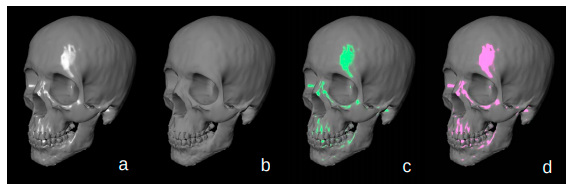
\includegraphics[width=15.0cm]{./img/SaturatedLowGloss.png}
            \caption{高彩度色の鏡面ハイライトによる光沢感の減衰の例}
            \label{SaturatedLowGloss}
        \end{figure}


    \section{本研究の目的}
        本研究では,色度情報が光沢感に寄与するかどうかを心理物理実験により明らかにすることを目的とする.
        また,色度情報による光沢感への寄与がある場合には,その寄与がどのようなメカニズムによって得られたかについても検討する.

    \section{本論文の構成}
        本論文の構成は以下の通りである.

        第1章では,研究背景として,光沢感に対する輝度情報の重要性について記すとともに,色度情報と光沢感の関連性に関する知見について記した.
        また,その背景に基づいた実験目的について記した.

        第2章では,光沢感知覚に色度情報が寄与するかどうかについて検討した実験1について記す.

        第3章では,実験1の結果に基づいて,光沢感と知覚的明るさとの関連性について記す.また,それらの関連性を詳細に検討するために実施した,知覚的明るさを計測する実験2について記す.

        第4章では,実験1と実験2の結果に基づいて,光沢感知覚に対する色度情報の寄与とそのメカニズムについて総合的に論ずる.

        第5章では,本研究から得られた成果についてまとめる.

    \newpage